\section{Dataset}

The dataset used to test the predictability of the developed model are about the COVID-19 oubreak in Italy. This dataset is used because the quarantine procedure has been implemented quite at the beginning of the outbreak, as in the model. Moreover Italy is a high-density country, especially in the Lombardy area, so that the small-world approximation may be feasible to describe the oubreak. Data in Italy and Lombardy are shown in Figures~\ref{fig:data_italy} and \ref{fig:data_lombardy}.\\

\begin{figure}[!ht]\centering
\subfloat[\label{fig:data_italy}]{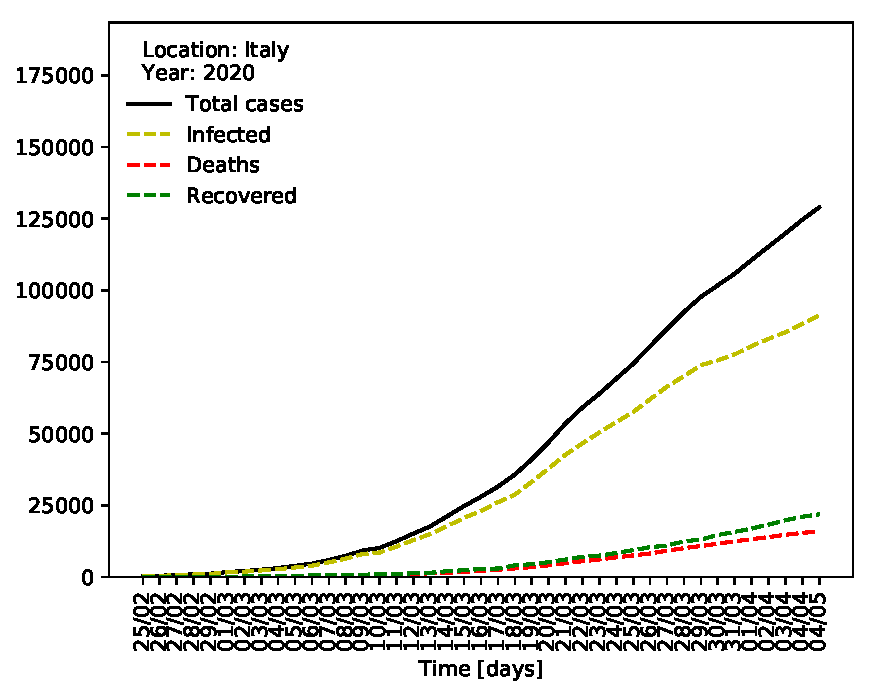
\includegraphics[width=0.4\textwidth]{imgs/Dataset/Data_Italy.pdf}}
\subfloat[\label{fig:data_lombardy}]{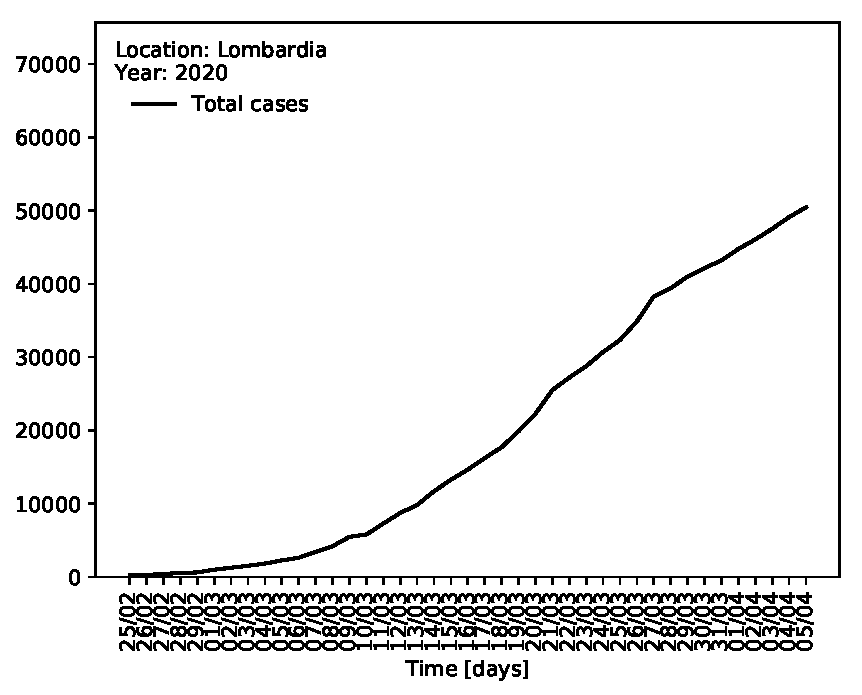
\includegraphics[width=0.4\textwidth]{imgs/Dataset/Data_Lombardia.pdf}}

\caption{Dataset collected in Italy (a) and Lombardy (b).}.
\end{figure}

A focus on Lombardy dataset is given, since it is by far the most affected region in Italy, completely driving the numbers of the outbreak in the whole country, and it is smaller, high-populated, very dynamic and connected area, where small-world approximation may work better.